\documentclass[10pt]{article}
\usepackage{icmlko}

\icmlmeta{IP 파운데이션 월드모델}{105}{넷째 축을 찾았다, 다만 틀린 채로}{입장료를 정렬에 넣으니 $+$0.0100으로 문턱에 가장 가까이 갔는데 --- 만화 · 세계애니에서 그 축은 가격이 아니라 연령 등급이었고, 개념을 바로잡자 악화 4/4가 됐다}

\begin{document}

\twocolumn[
\icmlheader

\begin{abstract}
노트 104가 단서를 남겼다 --- 사람이 정의한 공통 축 셋은 잔차 0.556으로 잘 맞으면서
쓸모가 있는데, 긁은 축은 잘 맞으면 중복이고(잔차 0.867 $\to$ $-$0.0130) 안 맞으면
정렬을 망친다(1.676). 그래서 넷째를 \emph{만들기} 전에 물었다 --- \textbf{이미
있지 않나.} \texttt{ALL5} 에는 다섯이 있는데 정렬에 쓰는 \texttt{COMMON} 은
셋뿐이다. \textbf{입장료와 미디어 홍보는 정의 불일치를 이유로 노트 20 · 22에서
빠졌고, 그 뒤로 아무도 다시 안 봤다.} 잔차를 재는 도구가 생겼으니 다시 봤다.
\textbf{입장료의 잔차는 0.980} --- 셋(0.556)보다 나쁘지만 긁은 축(1.676)보다
훨씬 낫다. 그대로 넣으면 $-$0.0003인데 \textbf{방향을 맞추면 $+$0.0100}이다.
라벨 상관이 팝업 $-$0.251 · 모바일 $-$0.371인데 만화 $+$0.549 · 세계애니
$+$0.587로 갈리기 때문이다. 방향은 보정 표본 50\%로 정직하게 정해도 $+$0.0106이
나오고(전체와 9.4/10 일치), 무작위로 뒤집으면 $-$0.0077이며, \textbf{방향만
맞추고 정렬에 안 넣으면 정확히 $+$0.0000}이다 --- 이득은 전적으로 \emph{넷째
공통 축}에서 온다. 씨앗 넷 구간의 하한이 $-$0.0019까지 올라왔다 ---
\textbf{이 프로젝트에서 채택 문턱에 가장 가까이 간 지렛대}다. 그런데 왜 부호가
갈리는지 보니 \textbf{만화 · 세계애니의 ``입장료''는 연령 등급}이었다. 개념을
바로잡아 가격이 아닌 넷을 끄자 잔차는 0.743으로 좋아지는데 판정치는
\textbf{$-$0.0262, 악화 4/4}다. \textbf{개념 정합과 예측력이 반대로 간다.}
\end{abstract}
]

\begin{figure*}[t]
\centering
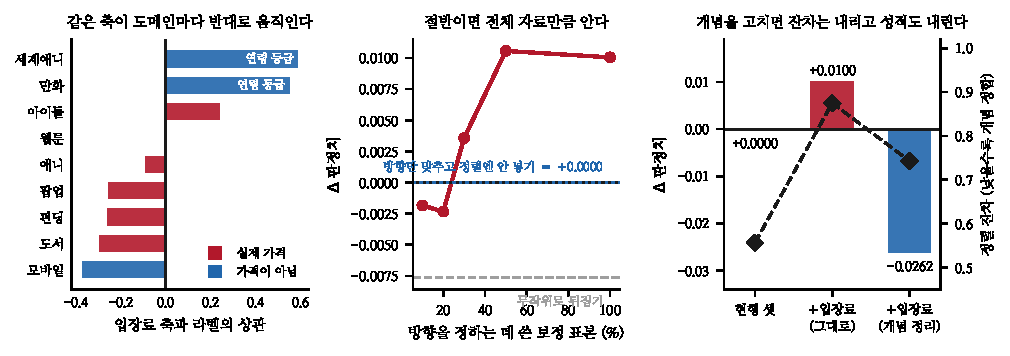
\includegraphics[width=\textwidth]{figs/f4.pdf}
\caption{왼쪽 --- 같은 축이 도메인마다 반대로 움직인다. 가운데 --- 절반이면
전체 자료만큼 안다. 오른쪽 --- 개념을 고치면 잔차는 내리고 성적도 내린다.}
\end{figure*}

\section{넷째는 이미 있었다}

정렬에 쓰는 축은 셋이다 --- 타깃 폭 · 굿즈 규모 · 매장 노출. \texttt{ALL5} 의
나머지 둘(입장료 · 미디어 홍보)은 노트 20 · 22에서 ``도메인 간 정의 불일치''를
이유로 빠졌고 그 뒤 여든 노트 동안 다시 검토된 적이 없다. 노트 103 · 104가
\textbf{잔차}라는 자를 만들었으니 그 판단을 다시 잰다.

\begin{table}[t]
\centering\tsize
\caption{정렬 잔차. 낮을수록 하나의 회전으로 맞출 수 있다.}
\begin{tabular}{lrr}
\toprule
& 잔차 & 쌍 \\
\midrule
굿즈 규모 & 0.512 & 72 \\
타깃 폭 & 0.565 & 88 \\
매장 노출 & 0.590 & 72 \\
\midrule
\textbf{입장료}(빠져 있음) & \textbf{0.980} & 72 \\
미디어 홍보(빠져 있음) & 0.727 & \textbf{6} \\
\midrule
긁은 축 emb0(노트 103) & 1.676 & 72 \\
\bottomrule
\end{tabular}
\end{table}

미디어 홍보는 다섯 도메인에서 덮개율 0\%라 쌍이 여섯뿐이다 --- 쓸 수 없다.
\textbf{입장료는 여덟 도메인에서 100\%이고 쌍이 72개다.}

\section{방향이 갈렸을 뿐이었다}

\begin{table}[t]
\centering\tsize
\caption{입장료 축과 라벨의 순위 상관.}
\begin{tabular}{lrlr}
\toprule
\multicolumn{2}{l}{\emph{음수 --- 값을 치른다}} &
\multicolumn{2}{l}{\emph{양수 --- 규모 신호}} \\
\midrule
모바일 & $-$0.371 & \textbf{세계애니} & \textbf{$+$0.587} \\
도서 & $-$0.293 & \textbf{만화} & \textbf{$+$0.549} \\
펀딩 & $-$0.257 & 아이돌 & $+$0.240 \\
팝업 & $-$0.251 & & \\
애니 & $-$0.089 & & \\
웹툰 & $-$0.003 & & \\
\bottomrule
\end{tabular}
\end{table}

\begin{table}[t]
\centering\tsize
\caption{정렬에 넣으면.}
\begin{tabular}{lrr}
\toprule
& $\rho$ & $\Delta$ \\
\midrule
현행 셋 & $+$0.4038 & --- \\
$+$입장료(그대로) & $+$0.4035 & $-$0.0003 \\
$+$미디어 홍보 & $+$0.4023 & $-$0.0015 \\
\textbf{$+$입장료 · 방향 맞춤} & \textbf{$+$0.4138} & \textbf{$+$0.0100} \\
\bottomrule
\end{tabular}
\end{table}

\claimx{입장료는 \textbf{정의 불일치가 아니라 방향 불일치}였다. 그대로 넣으면
$-$0.0003인데 도메인 여섯의 방향을 맞추면 $+$0.0100이다. 노트 20 · 22가 이
축을 뺀 판단은 여든 노트 동안 재검토된 적이 없었다.}{여섯 도메인의 방향을
라벨 상관으로 정했다. 다음 절이 그 누수를 막는다.}

\subsection{방향을 정직하게 정한다}

\begin{table}[t]
\centering\tsize
\caption{보정 표본에서만 방향을 정한다(노트 70의 절차). 씨앗 다섯 평균.}
\begin{tabular}{lrrr}
\toprule
보정 비율 & $\Delta$ & 팝업 & 전체와 일치 \\
\midrule
10\% & $-$0.0018 & $+$0.3521 & 8.8/10 \\
20\% & $-$0.0023 & $+$0.3639 & 8.4/10 \\
30\% & $+$0.0036 & $+$0.4144 & 9.2/10 \\
\textbf{50\%} & \textbf{$+$0.0106} & $+$0.4625 & 9.4/10 \\
100\%(전체) & $+$0.0100 & $+$0.4571 & 10/10 \\
\midrule
\multicolumn{2}{l}{\emph{대조}} & & \\
무작위로 뒤집기 & $-$0.0077 & $+$0.4212 & --- \\
\textbf{방향만 맞추고 정렬엔 안 넣기} & \textbf{$+$0.0000} & $+$0.4501 & --- \\
\bottomrule
\end{tabular}
\end{table}

\claimx{이득은 \textbf{전적으로 넷째 공통 축에서} 온다. 같은 방향 뒤집기를
하고 정렬에는 안 넣으면 $\Delta$ 가 \emph{정확히} $+$0.0000이다 --- 프로크루스테스가
고유 축의 부호를 알아서 흡수하기 때문이다. 그리고 방향은 절반의 표본이면
충분히 안다(9.4/10 일치).}{10 · 20\%에서는 음수다. 표본이 적으면 방향 추정이
틀리고, 틀린 방향은 안 넣느니만 못하다.}

\begin{table}[t]
\centering\tsize
\caption{채택 검정. 씨앗 넷 · 붓스트랩 100회.}
\begin{tabular}{lrl}
\toprule
& $\Delta$ & 95\% 구간 \\
\midrule
판정치 & $+$0.0100 & $[-0.0019,\ +0.0186]$ \\
& & $[-0.0030,\ +0.0183]$ \\
& & $[-0.0054,\ +0.0184]$ \\
& & $[-0.0054,\ +0.0192]$ \\
팝업 & $+$0.0070 & $[-0.0597,\ +0.1001]$ \\
\midrule
\multicolumn{3}{l}{\textbf{보류 4/4 --- 채택하지 않는다}} \\
\bottomrule
\end{tabular}
\end{table}

\claimx{구간 하한이 $-$0.0019까지 왔다. \textbf{노트 43 이후 채택 문턱에 가장
가까이 간 지렛대}다.}{그래도 넘지 못했다. 그리고 하한이 씨앗마다 $-$0.0019에서
$-$0.0054로 흔들리므로 ``거의 넘었다''를 강하게 읽으면 안 된다(노트 72의
씨앗 넷 규약이 정확히 이런 경우를 위한 것이다).}

\section{그런데 그 축은 가격이 아니었다}

부호가 왜 갈리는지 보려고 정의를 읽었다.

\begin{table}[t]
\centering\tsize
\caption{``입장료''가 실제로 재는 것.}
\begin{tabular}{lll}
\toprule
& 정의 & 타깃 폭과 상관 \\
\midrule
팝업 & 입장료(사람이 매김) & --- \\
애니 & 1화 대여 700원 & $-$0.005 \\
도서 & 정가 & --- \\
아이돌 & 앨범 정가 & --- \\
\midrule
\textbf{만화} & \textbf{전연령} & \textbf{$+$0.279} \\
\textbf{세계애니} & \textbf{전연령} & \textbf{$+$0.264} \\
웹툰 & 무료 & $-$0.026 \\
모바일 & 무료 & $-$0.064 \\
\bottomrule
\end{tabular}
\end{table}

\claimx{만화 · 세계애니의 입장료 축은 \textbf{가격이 아니라 연령 등급}이다 ---
그리고 타깃 폭이 이미 재는 것과 $+$0.27로 겹친다. 그 둘의 라벨 상관이
$+$0.55$\sim+$0.59로 유독 큰 이유가 이것이다. \textbf{$+$0.0100의 일부는
개념이 아니라 숫자를 맞춘 결과다.}}{웹툰 · 모바일은 ``무료''라 사실상 상수다.
상수 축은 주성분에 기여하지 않으므로 해가 없을 수도 있다.}

\begin{table}[t]
\centering\tsize
\caption{개념을 바로잡는다 --- 가격이 아닌 넷을 끈다.}
\begin{tabular}{lrr}
\toprule
& 잔차 & $\Delta$판정치 \\
\midrule
현행 셋 & 0.556 & --- \\
$+$입장료 · 방향 맞춤 & 0.875 & \textbf{$+$0.0100} \\
$+$입장료 · \textbf{가격 아닌 넷 끄기} & \textbf{0.743} &
\textbf{$-$0.0262} \\
\midrule
(끄기만 하고 정렬엔 안 넣음) & --- & $-$0.0314 \\
\bottomrule
\end{tabular}
\end{table}

\claimx{\textbf{개념 정합과 예측력이 반대로 간다.} 가격이 아닌 넷을 끄면 잔차가
0.875에서 0.743으로 좋아지는데 판정치는 $-$0.0262로 \textbf{악화 4/4}
($[-0.0342, -0.0148]$)다. 끄는 것 자체가 $-$0.0314이므로, ``틀린 것을 재던''
그 축이 네 도메인에서 실제로 쓸모가 있었다.}{연령 등급이 타깃 폭과 $+$0.27밖에
안 겹친다 --- 겹치지 않는 73\%가 진짜 정보일 수 있다. 그렇다면 그것은
\emph{입장료}가 아니라 이름 없는 다른 축이다.}

\begin{quote}\fontsize{9.5}{11.5}\selectfont
이 프로젝트가 같은 벽에 다섯 번째로 부딪힌다 --- \textbf{원리적으로 옳은 쪽이
진다.} 노트 40의 전역 정렬, 노트 48의 $\lambda$ 규칙, 노트 85--88의 공유
인코더, 노트 103의 공통 슬롯 승격, 그리고 여기. 매번 ``개념을 바로 세우는''
수정이 성적을 깎았다. \textbf{모형이 붙잡고 있는 것은 개념이 아니라 상관이다.}
\end{quote}

\section{한계}

\begin{itemize}[leftmargin=1.1em,itemsep=0.15em]
\item \textbf{채택 안 한다.} $+$0.0100이 보류 4/4다.
\item 방향을 보정 표본으로 정하는 절차가 50\%를 필요로 한다. 그만큼을 떼어
      놓으면 인자 공간이 얇아지는데 그 손실은 안 쟀다.
\item 만화 · 세계애니의 연령 등급이 무엇을 재는지 모른다. 타깃 폭과 겹치지
      않는 73\%의 정체가 미해결이다.
\item 미디어 홍보는 덮개율 때문에 판정 자체가 불가능하다. 다섯 도메인에서
      0\%다.
\item 시간 분할 판정(노트 77)을 이번에도 안 붙였다 --- 세 노트째 미룸.
\end{itemize}

\section{다음}

\begin{enumerate}[leftmargin=1.3em,itemsep=0.15em]
\item \textbf{이름을 다시 붙인다} --- 만화 · 세계애니의 연령 등급이 쓸모가
      있다면 그것은 ``입장료''가 아니라 \emph{접근 허용 폭}이다. 열 도메인에
      그 개념으로 다시 매기면 타깃 폭과 갈리는지 본다. 개념을 \emph{빼는} 대신
      \emph{바꾸는} 길이다.
\item \textbf{미디어 홍보의 덮개율을 채운다} --- 다섯 도메인에서 0\%인데,
      설명문 · 표지를 긁었듯이 홍보 신호(예고편 유무 · 공식 계정 · 보도)도
      긁을 수 있다. 잔차 0.727은 나쁘지 않았다.
\item $+$0.0100을 시간 분할로 다시 판정한다. 반쪽 검정과 달리 표본을 안 줄인다.
\item 팝업 표본. 모든 구간이 $n{=}75$ 에 걸려 있다.
\end{enumerate}

\vspace{0.6em}
\hrule height 0.3pt
\vspace{0.5em}
{\footnotesize
\textbf{참고문헌}\\[0.3em]
Meredith, W. (1993). Measurement invariance, factor analysis and factorial
invariance. \emph{Psychometrika}, 58(4), 525--543.\\[0.15em]
Schoenemann, P. H. (1966). A generalized solution of the orthogonal Procrustes
problem. \emph{Psychometrika}, 31(1), 1--10.\\[0.15em]
Ben-David, S. et al. (2010). A theory of learning from different domains.
\emph{Machine Learning}, 79(1--2), 151--175.\\[0.15em]
Little, R. J. A., Rubin, D. B. (2019). \emph{Statistical Analysis with Missing
Data}, 3rd ed. Wiley.\\[0.15em]
Efron, B., Tibshirani, R. J. (1993). \emph{An Introduction to the Bootstrap}.
Chapman \& Hall.
}

\end{document}
